% =====================================================================
%  EVO-X -- paper draft v2 (IEEE conference format), written against the
%  implemented Phase A-C system (package `evox`).
%
%  STATUS OF NUMBERS: the repository contains the complete implementation and
%  synthetic verification, but NO full real-data result runs yet.  Therefore
%  every results table below is filled automatically by `make_tables.py` from
%  a REAL, non-quick `evox compare` run, and shows a red TODO until then.
%  Never paste synthetic or --quick numbers into this paper.
%
%  Workflow:  run experiments -> python make_tables.py ... -> recompile ->
%             write the abstract/discussion from the real numbers.
%  Search for "TODO" before submission.
% =====================================================================
\documentclass[conference]{IEEEtran}

\usepackage[utf8]{inputenc}
\usepackage[T1]{fontenc}
\usepackage{cite}
\usepackage{amsmath,amssymb}
\usepackage{graphicx}
\usepackage{booktabs}
\usepackage{multirow}
\usepackage{xcolor}
\usepackage{algorithm}
\usepackage{algpseudocode}
\usepackage{tikz}
\usetikzlibrary{positioning,arrows.meta}
\usepackage[hidelinks]{hyperref}

\newcommand{\todo}[1]{\textcolor{red}{\textbf{[TODO: #1]}}}
\newcommand{\evox}{\textsc{EVO-X}}
\DeclareMathOperator*{\argmax}{arg\,max}
% result tables: use the generated file when present, otherwise a red TODO
\newcommand{\autotable}[2]{\IfFileExists{tables/#1.tex}{\input{tables/#1.tex}}{\todo{#2}}}

\begin{document}

\title{\evox: Governed Model Evolution for Continual Network Intrusion\\
Detection under Concept Drift}

\author{
\IEEEauthorblockN{Prashil Vilas Suryawanshi, Rameshwari Rajendra Satpute, Pooja Amol Bhosale, Himanshu Nitin Bangalkar}
\IEEEauthorblockA{Department of Computer Science and Engineering\\
Walchand College of Engineering, Sangli, India\\
Email: \todo{corresponding author email}}
\and
\IEEEauthorblockN{Leena V. Patil}
\IEEEauthorblockA{Department of Computer Science and Engineering\\
Walchand College of Engineering, Sangli, India}
}

\maketitle

% ---------------------------------------------------------------------
\begin{abstract}
Machine-learning intrusion detection systems (IDS) degrade after deployment as attacker and user behaviour change (concept drift). Existing continual-learning IDS provide effective adaptation mechanisms but usually apply one fixed pipeline whenever drift is detected, and seldom verify an updated model before it replaces the deployed one. We present \evox, a model-evolution management layer above a replaceable classifier. After drift is detected, \evox{} characterises it, a transparent two-stage controller (eligibility rules, then multi-objective utility ranking) selects one of five adaptation strategies to produce a \emph{candidate}, the candidate is evaluated on independent recent and historical holdouts, and a fail-closed safety gate decides promotion. Promoted models are versioned in a hash-chained append-only registry and monitored after deployment, with automatic restoration of the parent on degradation. We compare \evox{} with static, always-retrain, always-incremental, always-replay and two ``-inspired'' fixed-strategy baselines and three \evox{} ablations on six controlled drift scenarios, using separate validation and test seed families, seed-paired Holm-corrected tests and a predeclared non-inferiority margin. On real CICIDS2017 and UNSW-NB15 streams the multi-detector fusion front-end detects all injected drifts at a very low false-alarm rate and significantly beats every single detector; the controller, however, is so conservative that it behaves essentially like the static model, so none of our four maintenance hypotheses is supported after correction, and the advantage over a best fixed policy does not hold across datasets. We report these negative findings in full: the gate correctly screens most harmful candidates in a finite-horizon counterfactual, but with so few promotions this cannot be shown to matter in deployment.
\end{abstract}

\begin{IEEEkeywords}
intrusion detection, concept drift, continual learning, catastrophic forgetting, model governance, safe model updates
\end{IEEEkeywords}

% ---------------------------------------------------------------------
\section{Introduction}
Network IDS increasingly rely on classifiers trained on labelled flow datasets such as CICIDS2017~\cite{sharafaldin2018cicids} and UNSW-NB15~\cite{moustafa2015unsw}. The usual pipeline---train, deploy, predict---assumes the relation between flow features and labels is stationary. It is not: attackers change tools and timing and legitimate usage evolves, so the joint distribution shifts (concept drift~\cite{gama2014survey}) and an unadapted model silently loses detection capability.

Continual-learning IDS address this. SSF~\cite{zhang2024ssf} combines drift detection, strategic sample selection and forgetting; RepShield~\cite{liu2026repshield} protects old knowledge by projecting gradient updates away from a historical subspace; METANOIA~\cite{ying2025metanoia} targets lifelong host-level APT detection. These works improve the \emph{mechanics} of adapting. Two operational questions receive less attention for network-flow IDS: \emph{which} adaptation to use for a given drift rather than always the same one, and \emph{whether} an adapted model is safe to deploy. The second matters because an IDS that learns new attacks while forgetting old ones, or that raises false positives, can leave operators believing protection improved when it did not.

\evox{} treats model evolution as a governed decision problem. Drift is detected and characterised; a controller proposes one adaptation; the resulting candidate is never deployed directly but must pass independent evaluation and a safety gate; accepted models are versioned and monitored, and rolled back if they underperform. Unlike continual-learning IDS such as SSF~\cite{zhang2024ssf} and RepShield~\cite{liu2026repshield}, which commit to one fixed adaptation pipeline whenever drift is detected, and unlike retrain-timing work~\cite{pham2025retrain} that decides only \emph{whether} to retrain, \evox{} decides \emph{which} of several adaptation strategies to apply and gates the resulting model before it is deployed; we do not claim the individual mechanisms are new, only their governed combination.

\textbf{Contributions.}
\begin{enumerate}
  \item A governed evolution loop that links drift detection, drift characterisation, strategy selection, independent candidate evaluation, a fail-closed safety gate, versioned promotion and monitored rollback around a replaceable base classifier (Sec.~\ref{sec:method}).
  \item A transparent two-stage controller whose every decision is logged with its inputs, eligible set, utility terms and exclusions, with weights and gate thresholds chosen by a preregistered procedure on validation scenarios only (Sec.~\ref{sec:controller}, \ref{sec:gate}).
  \item A drift laboratory with six scenario types plus a drift-free control, recorded ground truth, disjoint validation/test pools, and a leakage-controlled closed-loop comparison protocol with source-group data roles and finite-horizon counterfactual measurement of harmful updates (Sec.~\ref{sec:setup}).
  \item An empirical comparison against fixed strategies and ablations on real CICIDS2017 and UNSW-NB15 streams, reporting per-scenario behaviour, harmful/unnecessary promotions and cost, in which the detector fusion clearly helps but the controller is found to be too conservative to improve on the static model --- a negative result we report in full (Sec.~\ref{sec:results}).
\end{enumerate}
We do not claim to have invented drift detection or continual learning, and we do not claim live deployment: experiments replay public benchmarks as streams.

% ---------------------------------------------------------------------
\section{Related Work}
\textbf{Concept drift.} Gama et~al.~\cite{gama2014survey} survey drift adaptation and fix the abrupt/gradual/incremental/recurring vocabulary used here. Cybersecurity-specific surveys~\cite{evolving2024survey} document how evolving environments challenge static IDS.

\textbf{Continual learning.} Continual learning is a stability--plasticity trade-off~\cite{wang2024cl}. SSF~\cite{zhang2024ssf} and RepShield~\cite{liu2026repshield} apply it to network IDS, each as one fixed pipeline; \evox{} treats such mechanisms as options a controller may choose from.

\textbf{Deciding when to retrain.} Pham et~al.~\cite{pham2025retrain} study when a deployed ML system should be retrained. They do not choose among adaptation types or validate candidate models.

\textbf{Lifelong IDS.} METANOIA~\cite{ying2025metanoia} treats lifelong operation as a design concern for provenance-based APT detection; we target network-flow IDS and add a multi-strategy controller and promotion gate.

\textbf{Online and active-learning IDS.} Camarda et~al.~\cite{camarda2025activedrift} combine an error-rate drift trigger with incremental Random Forest and uncertainty-based active learning, adapting only when drift is detected and labelling a small fraction of records to cut unnecessary retraining. Our active-incremental baseline follows this mechanism (incremental update on the least-confident released labels); \evox{} differs by choosing among several adaptation types and validating each candidate before deployment rather than updating on every trigger.

% ---------------------------------------------------------------------
\section{Problem Formulation}
\label{sec:problem}
Flows arrive in time-ordered batches with features $x$ and labels $y$. A deployed model $M_v$ scores each batch; labels for batch $t$ become available only after a delay of $k$ batches (and, optionally, for a labelled fraction). Drift occurs at unknown times. After an alarm the system chooses an action $a\in\mathcal{A}=\{\text{No-Op, Incremental, Replay, Strategic Selection, Full Retrain}\}$ to produce a candidate $M'$ from the parent $M_v$, and decides whether $M'$ replaces $M_v$. The objective is high detection quality on both recent and historical traffic with few updates, low adaptation cost and no harmful promotions.

% ---------------------------------------------------------------------
\section{The \evox{} Framework}
\label{sec:method}
\begin{figure}[t]
\centering
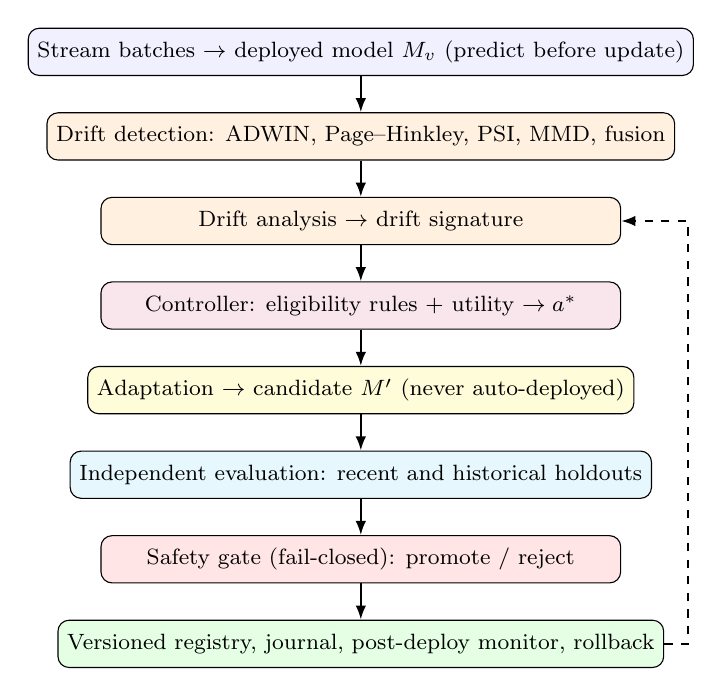
\begin{tikzpicture}[
  node distance=4.6mm,
  box/.style={draw, rounded corners, align=center, minimum width=6.6cm, minimum height=6mm, font=\footnotesize},
  arr/.style={-{Latex[length=1.8mm]}, thick}]
  \node[box, fill=blue!6] (s) {Stream batches $\rightarrow$ deployed model $M_v$ (predict before update)};
  \node[box, below=of s, fill=orange!12] (d) {Drift detection: ADWIN, Page--Hinkley, PSI, MMD, fusion};
  \node[box, below=of d, fill=orange!12] (a) {Drift analysis $\rightarrow$ drift signature};
  \node[box, below=of a, fill=purple!10] (c) {Controller: eligibility rules $+$ utility $\rightarrow a^{*}$};
  \node[box, below=of c, fill=yellow!15] (g) {Adaptation $\rightarrow$ candidate $M'$ (never auto-deployed)};
  \node[box, below=of g, fill=cyan!10] (e) {Independent evaluation: recent and historical holdouts};
  \node[box, below=of e, fill=red!10] (f) {Safety gate (fail-closed): promote / reject};
  \node[box, below=of f, fill=green!10] (r) {Versioned registry, journal, post-deploy monitor, rollback};
  \foreach \i/\j in {s/d,d/a,a/c,c/g,g/e,e/f,f/r}{\draw[arr] (\i) -- (\j);}
  \draw[arr, dashed] (r.east) -- ++(0.3,0) |- (a.east);
\end{tikzpicture}
\caption{The \evox{} loop. The dashed arrow denotes stored past signatures used for recurrence matching.}
\label{fig:arch}
\end{figure}

\subsection{Drift detection and fusion}
Four detectors are used, plus one extra label-free signal. ADWIN~\cite{bifet2007adwin} (River~\cite{montiel2021river}) monitors the per-flow error bits; Page--Hinkley~\cite{page1954ph} monitors the per-batch error rate; both observe labels only after the label delay. The Population Stability Index (PSI) compares a sliding window with the reference using reference-quantile bins and aggregates per-feature values by the mean of the five largest; MMD~\cite{gretton2012mmd} uses an RBF kernel with median-heuristic bandwidth on subsamples and a threshold calibrated on a disjoint half of the reference. PSI, MMD and ADWIN on prediction confidence need no labels. With normalised scores $s_i$ (1 = the detector's own threshold),
\begin{equation}
D_{\text{fused}}=\sum_i w_i\min(s_i,1),\qquad \sum_i w_i=1,
\end{equation}
and drift is declared on the rising edge of $D_{\text{fused}}\ge\theta$. Whether fusion reduces false alarms is measured rather than assumed (Sec.~\ref{sec:results}). Alarm time is the time the detector learns of the change, so error-based detectors include the label delay.

\subsection{Drift analysis}
Each alarm yields a \emph{drift signature} using at most $L$ batches after it (no look-ahead): magnitude (mean of PSI and MMD scores in units of their thresholds, capped), persistence (longest run above threshold), duration, an ``ended'' flag, a type guess, a confidence-based unfamiliarity score, the per-feature PSI vector, and recurrence (cosine similarity to stored past signatures). We found in the drift laboratory that confidence-based unfamiliarity rises under covariate shift as well as for new classes; it therefore only influences rule eligibility, never alone selects an action.

\subsection{Adaptation strategies and candidates}
Five strategies produce a candidate from the parent: \emph{No-Op} (returns the parent unchanged); \emph{Incremental} (Random Forest~\cite{breiman2001rf}: bounded prune-and-grow with explicit class-probability alignment; XGBoost~\cite{chen2016xgboost}: boosting continuation, available only if the class set is unchanged and fully represented, otherwise recorded as unavailable); \emph{Replay} (fresh model on recent data mixed with a bounded, class-balanced memory); \emph{Strategic Selection} (SSF-inspired: samples scored by error plus one minus confidence, each class kept represented, stale memory expired); and \emph{Full Retrain} on recent data only (the naive policy). Memory is bounded and class-balanced, and training uses only labels released under the label policy. A candidate records its parent, strategy, content-hashed training snapshot and measured resource profile; no adaptation changes the active model.

\subsection{Evolution controller}
\label{sec:controller}
\textbf{Stage 1: eligibility.} Given a signature with magnitude $m$, persistence $p$, recurrence $r$ and unfamiliarity $n$, the admissible set is given by Alg.~\ref{alg:rules}; No-Op is always available.
\begin{algorithm}[t]
\caption{Eligibility rules (thresholds $\tau$ are parameters)}
\label{alg:rules}
\begin{algorithmic}[1]
\If{$m<\tau_{\text{low}}$ \textbf{or} $p<\tau_{p,\text{short}}$ \textbf{or} ended} \State $E\gets\{\text{No-Op}\}$
\ElsIf{$r\ge\tau_{\text{rec}}$} \State $E\gets\{\text{Replay, Incremental, No-Op}\}$
\ElsIf{$n\ge\tau_{\text{nov}}$ \textbf{and} $m\ge\tau_{\text{high}}$} \State $E\gets\{\text{Retrain, Strategic, No-Op}\}$
\ElsIf{$m\ge\tau_{\text{high}}$ \textbf{and} $p\ge\tau_{p,\text{long}}$} \State $E\gets\{\text{Retrain, Replay, No-Op}\}$
\Else \State $E\gets\{\text{Incremental, Strategic, Replay, No-Op}\}$
\EndIf
\State remove unavailable actions and any action whose estimated training cost exceeds the budget
\end{algorithmic}
\end{algorithm}
The reported run froze these to the implemented defaults $\tau_{\text{low}}{=}1$, $\tau_{\text{high}}{=}3$, $\tau_{p,\text{short}}{=}2$, $\tau_{p,\text{long}}{=}10$, $\tau_{\text{rec}}{=}0.9$, $\tau_{\text{nov}}{=}0.2$, with controller utility weights (gain, forgetting, cost, FPR, latency) $=(0,0.5,0,0.5,0)$ and cost/latency scales $2.37$/$1.91$ selected on the validation seeds before the test scenarios were built.

\textbf{Stage 2: utility.} Among eligible actions,
\begin{align}
U(a)&=w_1\widehat{\Delta F1}(a)-w_2\widehat{\text{Forg}}(a)-w_3\widehat{\text{Cost}}(a)\nonumber\\
&\quad-w_4\widehat{\Delta\text{FPR}}(a)-w_5\widehat{\text{Lat}}(a),\\
a^{*}&=\argmax_{a\in E}U(a),
\end{align}
with ties broken toward No-Op, then lower cost. Gain, forgetting and $\Delta$FPR come from a cheap proxy evaluation on a small holdout (cheap candidates are trained on samples disjoint from the proxy set); cost and latency come from profiles frozen before test scenarios are built and are normalised by scale constants. Each decision record stores the signature, eligible set, exclusions with reasons, per-term utilities, weights and thresholds. Ablations: \emph{rules-only} (first eligible action) and \emph{utility-only} (all actions eligible).

\textbf{Preregistered weight selection.} Each $w_i\in\{0,0.25,0.5,1\}$, normalised and deduplicated. The selected vector maximises, on validation episodes only,
\begin{equation}
\overline{\tfrac12(F1_{\text{recent}}+F1_{\text{hist}})-\lambda\,\text{Cost}/c_0}
\end{equation}
($\lambda{=}0.05$), where outcomes are measured on an audit holdout independent of the proxy holdout; ties prefer lower cost. Test-family scenarios and seeds are refused by the code. The full sensitivity grid is reported.

\subsection{Independent evaluation and safety gate}
\label{sec:gate}
Candidates are evaluated on recent and historical holdouts excluded from their (and their ancestors') training data, measuring recent gain $\Delta F1_{\text{new}}$, historical change $\Delta F1_{\text{hist}}$, forgetting versus the best historical per-class scores, $\Delta$FPR, training cost and inference latency. The gate promotes only if all of
\begin{equation}
\begin{aligned}
&\Delta F1_{\text{new}}\ge\tau_1,\ \Delta F1_{\text{hist}}\ge-\tau_2,\ \text{Forg}\le\tau_3,\\
&\Delta\text{FPR}\le\tau_4,\ \text{Train}\le\tau_5,\ \text{Lat}\le\tau_6
\end{aligned}
\end{equation}
hold; missing, non-finite or physically invalid metrics reject (fail-closed), and rejection leaves the active model untouched. Thresholds are selected from a preregistered 48-point grid ($\tau_1\!\in\!\{0,.01,.02\}$, $\tau_2\!\in\!\{.02,.05\}$, $\tau_3\!\in\!\{.03,.1\}$, $\tau_4\!\in\!\{.005,.02\}$, $\tau_5\!\in\!\{B/2,B\}$) using one-step validation pilots and independent audit outcomes, then frozen before test scenarios exist; the pilots keep the initial parent fixed and are not reported as deployed performance. An optional retry with an alternative strategy is not enabled.

\subsection{Registry, monitoring and rollback}
Each policy owns a file registry of versioned, checksum-verified model artifacts and an append-only, fsynced, sequence-checked, hash-chained event journal (candidates, decisions, snapshots, parameters, drift context, pointer changes). Replaying the journal reconstructs the deployed version; damaged journals fail closed, and an exclusive lease rejects competing owners. Version states are \texttt{CANDIDATE}, \texttt{DEPLOYED}, \texttt{SUPERSEDED}, \texttt{REJECTED} and \texttt{ROLLED\_BACK}. After promotion the in-memory model holder is swapped atomically; a monitor compares the new model with its frozen parent on fresh labelled monitor rows (default: two batches and 32 rows) and an independent historical anchor, and restores the parent if performance or FPR degrades.

% ---------------------------------------------------------------------
\section{Experimental Setup}
\label{sec:setup}
\subsection{Data and streams}
Primary dataset: CICIDS2017~\cite{sharafaldin2018cicids}; cross-dataset evaluation on UNSW-NB15~\cite{moustafa2015unsw} was run with Random Forest (Sec.~\ref{sec:generality}). Flows are time-ordered by timestamp; the reference window is the first $30\%$ of the deduplicated stream ($20\%$ of it held out for validation), and the standardiser is fit on the reference-training split only (verified mean~$\approx0$, std~$\approx1$). The exact source is the original CICIDS2017 \texttt{TrafficLabelling} (``GeneratedLabelledFlows'') release; after deduplication the CICIDS2017 stream has $2{,}234{,}468$ flows over $13$ classes and $21$ features, and the UNSW-NB15 stream has $2{,}024{,}668$ flows over $10$ classes and $38$ features.

\subsection{Drift scenarios}
Because natural CICIDS2017 drift is almost entirely novel-class drift, known-class drift is constructed. Six scenario types (abrupt, gradual, recurring, temporary, incremental, novel-class) plus a drift-free control are generated from a class-indexed pool of real flows with recorded ground truth. Class-mix changes are prior shift and bounded feature offsets on informative features are synthetic covariate shift; their combination is \emph{synthetic} concept drift. Low/medium/high magnitudes change strength, not which classes or features shift. Validation and test scenarios use disjoint flow pools and different seeds (3 validation, 6 test seeds). Table~\ref{tab:calib} calibrates the injected drift on the real stream: the static model's error rises from $\approx\!0.6\%$ before drift to a scenario-dependent level afterwards, and the mean post-drift error grows monotonically with magnitude ($0.10$, $0.14$, $0.20$ for low/medium/high, averaged over kinds). Temporary and abrupt shifts hurt the static model most, while the novel-class calibration barely changes its macro-F1 because the injected novel share is small at this stage.
\begin{table}[t]
\centering\caption{Magnitude calibration on real CICIDS2017 flows (medium magnitude): static-model error and macro-F1 drop before vs.\ after injected drift.}\label{tab:calib}
\footnotesize
\begin{tabular}{lccc}
\toprule
Drift kind & Err.\ pre & Err.\ post & Macro-F1 drop \\
\midrule
Abrupt      & 0.006 & 0.213 & 0.144 \\
Gradual     & 0.006 & 0.073 & 0.053 \\
Recurring   & 0.006 & 0.090 & 0.023 \\
Temporary   & 0.006 & 0.308 & 0.178 \\
Incremental & 0.006 & 0.078 & 0.053 \\
Novel-class & 0.006 & 0.086 & $-0.004$ \\
\bottomrule
\end{tabular}
\end{table}

\subsection{Closed-loop protocol and data roles}
All policies share the initial model, source flows, label access, windows and alarms from a frozen initial sentinel detector; each then evolves its own deployed model. Predictions are made before any update. Repeated appearances of an original source flow stay in one role even under different drift offsets: 50\% training, 15\% proxy, 15\% gate, 10\% monitor and 10\% report; historical validation samples are class-stratified into the four evaluation roles. Report rows influence nothing: they are used retrospectively for final metrics. Labels follow a delayed (and/or fractional) policy uniformly across all systems, $k=2$ batches.

\subsection{Systems}
Ten policies are compared (Table~\ref{tab:systems}). Fixed policies deploy any valid candidate unconditionally and have no gate or rollback; the \evox{} variants use monitoring, and all but \evox-no-gate use the safety gate. Unsupported XGBoost class-expansion updates are recorded as unavailable and not silently replaced by retraining. ``-inspired'' baselines are approximations of the cited mechanisms, not reproductions.
\begin{table}[t]
\centering\caption{Compared policies.}\label{tab:systems}
\footnotesize
\begin{tabular}{ll}
\toprule
Policy & Behaviour at every alarm\\
\midrule
Static & never updates\\
Always Retrain / Incremental / Replay & fixed action, deployed unconditionally\\
SSF-inspired & strategic selection with expiry, fixed\\
Active-incremental & incremental on least-confident half of released labels\\
\evox{} & rules $+$ utility, gate, monitor\\
\evox{} no gate & as \evox{} without the pre-deployment gate\\
\evox{} rules-only / utility-only & controller ablations\\
\bottomrule
\end{tabular}
\end{table}

\subsection{Metrics}
Accuracy is not a headline metric. We report macro-F1 and per-class detection, historical-anchor forgetting and backward transfer, a binary novel-class forward-transfer proxy (not a full task-matrix score), recovery time (two attack-supported batches within 0.02 of pre-drift binary F1; unrecovered events are censored), training/proxy wall and CPU time, sampled process RSS, Python allocation peak, model size, inference latency, and lifecycle counts (updates, rejections, rollbacks, unavailable updates).

\textbf{Harmful and unnecessary updates.} Frozen candidates and parents are shadow-scored on ten future reporting batches after labels arrive. A promoted or rejected candidate is \emph{harmful} if deploying it would lower future or historical macro-F1 by more than 0.03, and a promoted update is \emph{unnecessary} if its future gain is below 0.01. Empty horizons are censored and truncated ones flagged. This is a finite-horizon frozen-parent counterfactual, not a replay of the whole alternative trajectory.

\subsection{Hypotheses and statistics}
\begin{itemize}
  \item \textbf{H1} strategy selection improves detection relative to fixed policies;
  \item \textbf{H2} \evox{} performs fewer updates than always-retrain while macro-F1 stays within 0.02 of the best fixed policy;
  \item \textbf{H3} the gate reduces harmful promotions versus the no-gate ablation;
  \item \textbf{H4} \evox{} shows less historical forgetting than recent-only full retraining.
\end{itemize}
Scenarios are averaged within each seed before testing (no pseudo-replication). Paired Wilcoxon signed-rank tests use Holm correction~\cite{wilcoxon1945,holm1979}; H2 additionally uses a one-sided non-inferiority test with margin 0.02. With fewer than six paired seeds no test is run, and any hypothesis is reported as supported, not supported or inconclusive by predeclared rules; synthetic or quick runs are always inconclusive. Algorithm portability (RQ6) and cross-dataset generality (RQ7) are reported in Sec.~\ref{sec:generality}.

\subsection{Implementation and verification}
\evox{} is implemented in Python (scikit-learn, XGBoost, River, Kafka/in-memory transport). The test suite (207 tests) covers data-role isolation, gate boundaries, candidate/parent identity, journal integrity and rollback, including prediction-identical restoration of the parent after rejection and promotion and recovery after reopening the registry. These tests verify mechanism correctness, not detection performance. A Kafka replay is checked to be bit-identical to in-memory scoring by an automated test rather than by a separate benchmark. On the in-memory transport the end-to-end per-batch latency (500 flows) is $14.4$~ms mean ($19.8$~ms p95) for Random Forest and $8.7$~ms ($13.1$~ms p95) for XGBoost, i.e.\ roughly $29$ and $17$~ms per~1000 flows, well within the $100$~ms/1000-flow budget.

% ---------------------------------------------------------------------
\section{Results}
\label{sec:results}
All numbers in this section come from the real CICIDS2017 run (\texttt{data\_tag=REAL}, algorithm Random~Forest unless stated, detector parameters tuned on three validation seeds, results on the six test seeds 2001--2006; 114 test scenarios), with XGBoost and UNSW-NB15 used for the generality study (Sec.~\ref{sec:generality}). The run stores the frozen protocol, configuration, source-data hashes and a source snapshot. The headline finding is negative and is reported as such: the multi-detector front-end is strong, but on these streams the \evox{} controller is conservative to the point of behaving almost exactly like the static model, and no hypothesis is supported after Holm correction over six seeds.

\subsection{Drift detection}
On the test scenarios, every single detector misses some events, and the three error- and distribution-based members disagree about which (Table~\ref{tab:detectors}). The weighted fusion detects all 126 events (detection rate $1.000$) at the lowest false-alarm rate ($0.15$ per~1000 batches), at the cost of a short mean delay ($3.57$ batches) inherited from the slower members; PSI alone is fastest (median delay $0$) but misses part of the novel-class drift that error-based members catch once labels arrive. Fusion dominates each member on detection fraction, and the paired Wilcoxon tests reject equality against all five members ($p<0.003$); its false-alarm advantage is significant against ADWIN-err, PH-err and MMD but not against the already clean PSI and ADWIN-conf.
\begin{table}[t]
\centering\caption{Detector comparison on test scenarios (parameters tuned on validation only).}\label{tab:detectors}
\footnotesize\resizebox{\columnwidth}{!}{\autotable{detectors}{run Phase A on the real stream, then make\_tables.py --detector-csv}}
\end{table}

\subsection{Strategy selection versus fixed policies}
\begin{table*}[t]
\centering\caption{Closed-loop comparison on test scenarios (mean $\pm$ std over scenario/seed runs).}\label{tab:main}
\footnotesize\autotable{comparison}{run `evox compare` on the real stream (full mode), then make\_tables.py --compare-dir}
\end{table*}

\begin{table}[t]
\centering\caption{Seed-paired comparisons of \evox{} against each baseline (Holm-adjusted).}\label{tab:paired}
\footnotesize\resizebox{\columnwidth}{!}{\autotable{paired}{paired\_statistics.csv}}
\end{table}

Two results stand out (Table~\ref{tab:main}). First, \emph{unconditional updating is a mixed strategy, not a free win}: on these streams the fixed incremental and replay policies raise macro-F1 over the static model (to $0.744$ and $0.728$ from $0.700$) but at the price of historical forgetting ($0.080$ and $0.013$), while always-retrain and the SSF-inspired policy \emph{lower} macro-F1 (to $0.720$ and $0.588$) and forget the most ($0.208$ and $0.449$). Second, \evox{} is extremely conservative: it promotes $0.04$ models per scenario on average, so its macro-F1 ($0.701$), binary F1, FPR and forgetting are statistically indistinguishable from the static model, and it leaves the gains that the fixed incremental policies collect on the table. The per-drift-type breakdown (available in \texttt{per\_scenario.csv}) locates the gap: all policies, \evox{} included, lose the most macro-F1 on novel-class drift (static $0.554$; best fixed $\approx0.68$), and \evox{}'s few promotions recover almost none of it. Where a fixed policy is already near-optimal (recurring, gradual) the cost of not updating is small; where adaptation would help most (novel-class, temporary) \evox{} does not act. The seed-paired tests (Table~\ref{tab:paired}) make the same point quantitatively: although \evox{} uses far fewer updates and forgets far less than the fixed policies, \emph{no} comparison survives Holm correction over six seeds (all adjusted $p\ge0.14$), so none of these differences is claimed as significant.

\subsection{Safety gate and counterfactual harm}
The finite-horizon counterfactual (Table~\ref{tab:cf}) shows the gate acting as intended on the candidates it does see: the rules-only controller, which proposes many candidates ($106$), would deploy $83$ harmful ones if unchecked, whereas full \evox{} proposes only $9$ ($5$ harmful) and its gate plus utility term keep almost all of them out of deployment. A 48-configuration threshold sweep on validation data accepts between $37$ and $103$ candidates (harmful accepted $1$--$17$), so the gate is neither vacuous nor degenerate: it does reject, and its strictness is controllable. The caveat is that over six test seeds the gate-versus-no-gate difference in \emph{deployed} harmful promotions ($0.01$ vs.\ $0.04$) is too small to be significant, so H3 remains inconclusive despite the clear counterfactual signal.
\begin{table}[t]
\centering\caption{Finite-horizon counterfactual outcomes of candidates.}\label{tab:cf}
\footnotesize\resizebox{\columnwidth}{!}{\autotable{counterfactual}{counterfactuals.csv}}
\end{table}

\subsection{Ablations}
Removing the gate (\evox{} no-gate) barely changes behaviour because the controller already selects No-Op on almost every alarm (updates rise only from $0.04$ to $0.08$ per scenario). The two controller halves behave differently: rules-only is the most active variant ($0.23$ updates, $0.70$ rejections per scenario) and the only one whose counterfactual harm is large, while utility-only sits in between; both leave macro-F1 within $0.01$ of \evox{} and static. The practical reading is that on these streams the utility term, not the gate, is what suppresses updates, and it suppresses them so aggressively that the full system degenerates toward the static policy.

\subsection{Hypothesis assessment}
Under the predeclared rules, all four hypotheses are \emph{inconclusive} on the real run (Table~\ref{tab:hyp}): with six paired seeds the Holm-corrected tests have too little power, and the controller's near-static behaviour means the effects they test for are small to begin with. We report this plainly rather than selecting an uncorrected comparison. The same statuses hold for the XGBoost run.
\begin{table}[t]
\centering\caption{Hypothesis status under the predeclared rules.}\label{tab:hyp}
\footnotesize\resizebox{\columnwidth}{!}{\autotable{hypotheses}{hypotheses.json}}
\end{table}

\subsection{Algorithm and dataset generality}
\label{sec:generality}
\textbf{Random Forest vs.\ XGBoost.} Repeating the full protocol with XGBoost (controller logic unchanged) reproduces the pattern: static macro-F1 $0.731$, best fixed $0.777$ (always-replay), and \evox{} $0.735$ --- again essentially the static model, with $0.14$ updates per scenario and all four hypotheses inconclusive. A cross-algorithm transfer check (train the controller on Random Forest, apply to XGBoost) gives native \evox{} $0.7346$ versus transferred $0.7325$ and static $0.7309$, with $90.4\%$ action agreement; because the native controller does not beat static, H5 (transferability of a learned advantage) is inconclusive --- there is no advantage to transfer.

\textbf{UNSW-NB15.} On UNSW-NB15 (Random Forest, six seeds) \evox{} reaches macro-F1 $0.524$ against a best-fixed $0.577$, an advantage of $-0.054$, slightly worse than the CICIDS2017 reference gap of $-0.049$; by the pre-registered criterion (same-sign advantage within $50\%$ of the reference) the \evox{}-vs-best-fixed result does \emph{not} hold across datasets. The one robust cross-dataset finding is relative: \evox{} beats the weak SSF-inspired baseline on both datasets and across every drift kind ($+0.113$ on CICIDS2017, $+0.118$ on UNSW-NB15). Per drift kind the sign of \evox{}'s advantage over the best fixed policy is mostly negative on both datasets, with the largest deficits on novel-class drift ($-0.130$ and $-0.110$). The advantage is never averaged across datasets.

% ---------------------------------------------------------------------
\section{Discussion}
The results are a mix of one clear positive and one clear negative, and we state both. The positive is the detection front-end: weighted fusion of heterogeneous detectors catches every injected change at a very low false-alarm rate and significantly dominates each individual detector, confirming that no single drift signal is sufficient on these streams. The negative, and the more important finding, is that the \evox{} controller as configured is \emph{too conservative to demonstrate a benefit}. On every setting we ran --- Random Forest and XGBoost, CICIDS2017 and UNSW-NB15 --- the controller selects No-Op on almost all alarms, so the deployed model tracks the static model and never collects the gains that a plain always-incremental policy obtains. Consequently none of H1--H4 is supported, H5 is moot, and the safety claims hold only in the trivial sense that a system which rarely updates rarely deploys a harmful update.

The counterfactual analysis clarifies \emph{why} this is not simply a broken gate. When the controller does propose candidates (the rules-only ablation), the gate correctly screens out the large majority of harmful ones, and the validation sweep shows the gate is tunable rather than vacuous. The bottleneck is upstream: on these streams the utility term, driven by cautious proxy estimates of future gain, judges most candidates not worth deploying, and because real improvements over static are themselves small (novel-class drift aside) this caution is hard to distinguish from correct behaviour. Whether the controller is appropriately or excessively conservative cannot be settled with six seeds; it is the central open question these runs raise. We also note the mismatch between the strong per-candidate counterfactual signal and the non-significant seed-level tests, which is a power problem, not a contradiction.

\subsection{Limitations}
\begin{itemize}
  \item Public benchmark streams, not live deployment; the datasets are dated and have known labelling artefacts, so results are relative comparisons.
  \item Most drift is synthetic (re-sequenced class mix plus bounded offsets); real drift may differ.
  \item Few base models (Random Forest, XGBoost); other architectures untested.
  \item Controller weights and gate thresholds are domain dependent; we report sensitivity, not a universal optimum.
  \item ``-inspired'' baselines are re-implementations of the cited mechanisms.
  \item Harm is measured by a finite-horizon frozen-parent counterfactual, not a full alternate trajectory.
  \item Six test seeds can be underpowered after Holm correction.
  \item The forward-transfer score is a binary proxy and memory figures mix Python allocation peaks with sampled process RSS.
  \item Confidence-based unfamiliarity is not specific to new classes; on the real run the confidence detector had the weakest novel-class detection of all members ($0.39$), consistent with this.
\end{itemize}

% ---------------------------------------------------------------------
\section{Conclusion}
We built and verified a closed-loop IDS maintenance framework and evaluated it on real CICIDS2017 and UNSW-NB15 streams with Random Forest and XGBoost. The multi-detector fusion front-end is a solid positive result: it detects all injected drifts at a very low false-alarm rate and significantly beats every single detector. The controller result is negative and reported as such: on all settings tried, \evox{} is so conservative that it behaves essentially like the static model, so none of the four maintenance hypotheses is supported after Holm correction over six seeds, cross-algorithm transfer offers no advantage to carry, and the \evox{}-vs-best-fixed advantage does not hold from CICIDS2017 to UNSW-NB15. The safety gate screens out most harmful candidates in the finite-horizon counterfactual and is tunable, but with so few promotions this cannot be shown to matter in deployment. Future work therefore targets the controller's caution directly --- recalibrated proxy estimates and utility weights, more seeds and magnitudes for statistical power, meta-learned strategy selection, cross-dataset and federated deployment, and robustness to adversarial drift that targets the controller.

\section*{Reproducibility}
Code, tests and configuration are in the project repository (\url{https://github.com/RameshwariS/EVO_X}); the reported runs are at commit \texttt{6a63238}. Dependencies are pinned through \texttt{pyproject.toml} (scikit-learn, XGBoost, River). The frozen controller, gate and label-policy configuration (utility weights, signature thresholds and seeds) is stored with each run as \texttt{frozen\_controller.json} and \texttt{preregistered\_protocol.json}, written before the test scenarios were built; validation seeds are 1001--1003 and test seeds 2001--2006. Each run directory also stores the source-data SHA-256 hashes and a source snapshot, so the stream can be rebuilt and the comparison re-run with the recorded one-command pipeline.

\section*{Acknowledgment}
We thank our project guide for continued supervision, and an external reviewer who gave detailed feedback on the project synopsis that sharpened the controller design, the choice of baselines and the experimental protocol.

\bibliographystyle{IEEEtran}
\bibliography{references}
\end{document}